\section{Masking}
\nblink{brats/16\_brats\_hausdorff\_masks\_examples.ipynb}

The first part of the algorithm is the occlusion of parts of the input image.
We iterate over the image in a linear fashion, from left to right and from top to bottom, based on an pixel offset between every row and column defined as a parameter of the algorithm.
For every position that is encountered, we create a new image. On this image, we draw a filled black circle at the specific position.
Some examples of this changed images are shown in Figure \ref{hdm_masks_1} and \ref{hdm_masks_2}.

We chose the circle shape (instead of a square), because many objects visible in medical imaging and real world images are round, and not squares.
The current implementation only supports the complete removal of information (setting all pixel values to zero) inside the circle, but other approaches like
setting the color to the mean value of the pixels inside the circle, setting all the pixel to 1 (full intensity) might also work.
The size of the circle is a configuration parameter of the algorithm, some experimentation of different sizes is done in \autoref{hdm_circle_size}.

The drawing of the black circle is implemented in a similar way to RISE. As a first step, masks with the black circles are generate. In a second step,
these masks are applied to the images. The generation of the masks is not very slow, but the masks are exactly the same for the same parameters of the algorithm and therefore
only need to be generated once.

The masks are generated based on the image size and the configured offset between the circles.
This is done by creating an image with the same width and height of the input image using the Python Imaging Library (PIL). All pixels are set to full intensity (white) on initialization.
The PIL draw module is then used to draw the black circle onto the image. As a last step, the image in converted into a numpy array. This process is repeated for all positions generated
by the offset parameter of the algorithm.

Applying the mask to and image is done using the numpy \texttt{min()} function with the mask and the image as a parameter giving an output looking like Figure \ref{hdm_masks_1} and \ref{hdm_masks_2}.

\begin{figure}[H]
    \centering
    \begin{subfigure}[t]{.33\textwidth}
        \centering
        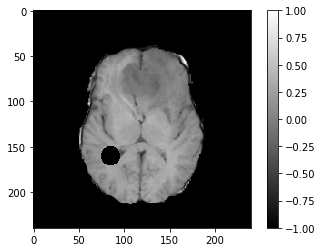
\includegraphics[width=\linewidth]{chapters/06_hdm/images_masked/masked_0.png}
        \caption{T1 modality with mask applied}
    \end{subfigure}%
    \begin{subfigure}[t]{.33\textwidth}
        \centering
        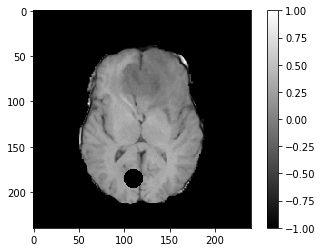
\includegraphics[width=\linewidth]{chapters/06_hdm/images_masked/masked_4.png}
        \caption{T1 modality with a different mask applied}
    \end{subfigure}
    \begin{subfigure}[t]{.33\textwidth}
        \centering
        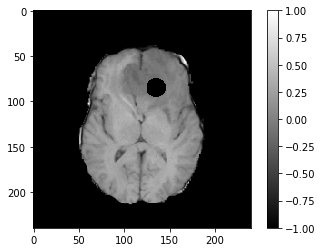
\includegraphics[width=\linewidth]{chapters/06_hdm/images_masked/masked_8.png}
        \caption{T1 modality with a third mask applied}
    \end{subfigure}
    \caption{Modality T1 with three different round masks applied}
    \label{hdm_masks_1}
\end{figure}

\begin{figure}[H]
    \centering
    \begin{subfigure}[t]{.33\textwidth}
        \centering
        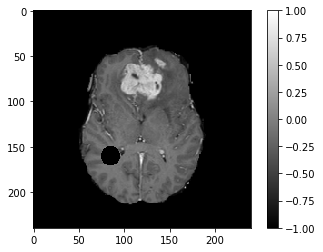
\includegraphics[width=\linewidth]{chapters/06_hdm/images_masked/masked_1.png}
        \caption{T1 enhanced contrast modality with mask applied}
    \end{subfigure}%
    \begin{subfigure}[t]{.33\textwidth}
        \centering
        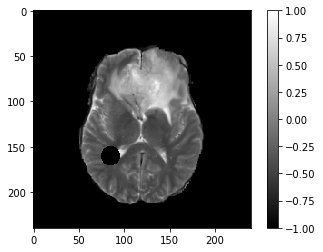
\includegraphics[width=\linewidth]{chapters/06_hdm/images_masked/masked_2.png}
        \caption{T2 modality with mask applied}
    \end{subfigure}
    \begin{subfigure}[t]{.33\textwidth}
        \centering
        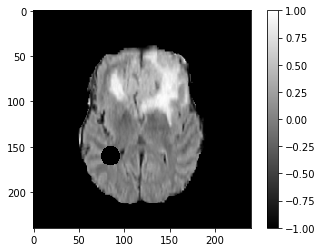
\includegraphics[width=\linewidth]{chapters/06_hdm/images_masked/masked_3.png}
        \caption{FLAIR modality with mask applied}
    \end{subfigure}
    \caption{Modalities T1 contrast enhanced, T2 and FLAIR with the same mask applied}
    \label{hdm_masks_2}
\end{figure}



\section{Changed segmentation output}
The images with the masks applied from above are then run trough the neural networks. As seen in Figure \ref{hdm_changed_output_1}, the output segmentation may not change or only change slightly when applied to an unimportant part of the image. Applying the mask on important parts of the image can change the segmentation output significantly, as seen in Figure \ref{hdm_changed_output_2}, \ref{hdm_changed_output_3} and \ref{hdm_changed_output_4}.

\begin{figure}[H]
    \centering
    \begin{subfigure}[t]{.33\textwidth}
        \centering
        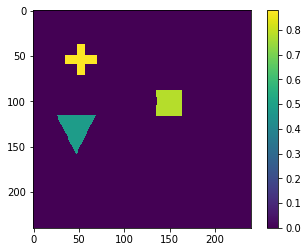
\includegraphics[width=\linewidth]{chapters/06_hdm/images_analyze/1a_masked.png}
        \caption{Input with mask applied on the left side of the square}
    \end{subfigure}%
    \begin{subfigure}[t]{.33\textwidth}
        \centering
        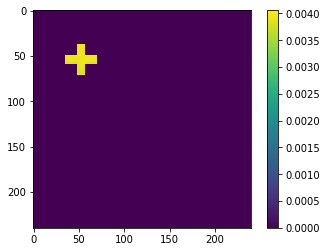
\includegraphics[width=\linewidth]{chapters/06_hdm/images_analyze/1b_segment.png}
        \caption{Changed output segment}
    \end{subfigure}
    \begin{subfigure}[t]{.33\textwidth}
        \centering
        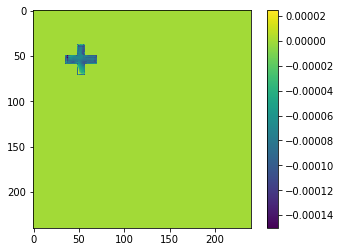
\includegraphics[width=\linewidth]{chapters/06_hdm/images_analyze/1c_diff.png}
        \caption{Difference of the new output segment to the reference output segment (reference output - new output segment)}
    \end{subfigure}
    \caption{The input image (a) is only slightly changed by drawing a circle on the left side of the square. The segment output (b) looks the same as the reference output. The difference with the reference output shows that the segment changed, the confidence for the segment output even increased, but only by a very small amount. }
    \label{hdm_changed_output_1}
\end{figure}

\begin{figure}[H]
    \centering
    \begin{subfigure}[t]{.33\textwidth}
        \centering
        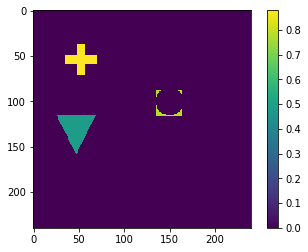
\includegraphics[width=\linewidth]{chapters/06_hdm/images_analyze/0a_masked.png}
        \caption{Input with mask applied on the top left side of the cross}
    \end{subfigure}%
    \begin{subfigure}[t]{.33\textwidth}
        \centering
        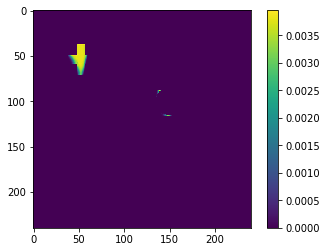
\includegraphics[width=\linewidth]{chapters/06_hdm/images_analyze/0b_segment.png}
        \caption{TODO}
    \end{subfigure}
    \begin{subfigure}[t]{.33\textwidth}
        \centering
        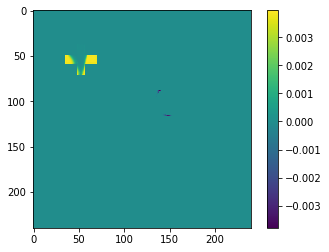
\includegraphics[width=\linewidth]{chapters/06_hdm/images_analyze/0c_diff.png}
        \caption{TODO}
    \end{subfigure}
    \caption{TODO}
    \label{hdm_changed_output_2}
\end{figure}

\begin{figure}[H]
    \centering
    \begin{subfigure}[t]{.33\textwidth}
        \centering
        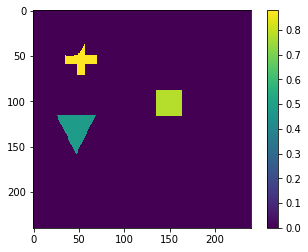
\includegraphics[width=\linewidth]{chapters/06_hdm/images_analyze/3a_masked.png}
        \caption{TODO}
    \end{subfigure}%
    \begin{subfigure}[t]{.33\textwidth}
        \centering
        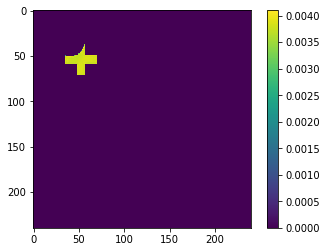
\includegraphics[width=\linewidth]{chapters/06_hdm/images_analyze/3b_segment.png}
        \caption{TODO}
    \end{subfigure}
    \begin{subfigure}[t]{.33\textwidth}
        \centering
        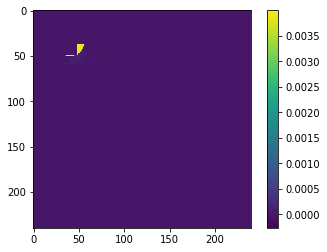
\includegraphics[width=\linewidth]{chapters/06_hdm/images_analyze/3c_diff.png}
        \caption{TODO}
    \end{subfigure}
    \caption{TODO}
    \label{hdm_changed_output_3}
\end{figure}


\begin{figure}[H]
    \centering
    \begin{subfigure}[t]{.33\textwidth}
        \centering
        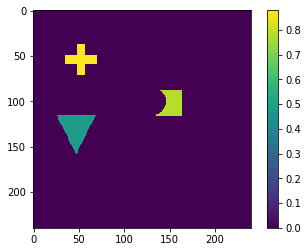
\includegraphics[width=\linewidth]{chapters/06_hdm/images_analyze/2a_masked.png}
        \caption{Input with mask applied on the left side of the square}
    \end{subfigure}%
    \begin{subfigure}[t]{.33\textwidth}
        \centering
        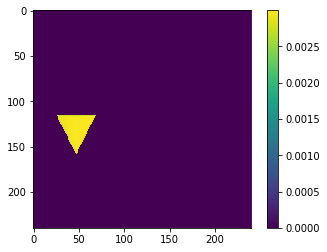
\includegraphics[width=\linewidth]{chapters/06_hdm/images_analyze/2b_segment.png}
        \caption{Changed output segment}
    \end{subfigure}
    \begin{subfigure}[t]{.33\textwidth}
        \centering
        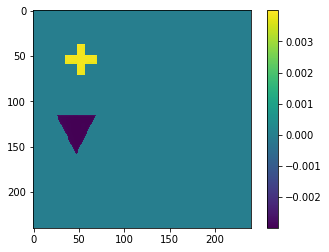
\includegraphics[width=\linewidth]{chapters/06_hdm/images_analyze/2c_diff.png}
        \caption{Difference of the new output segment to the reference output segment (reference output - new output segment)}
    \end{subfigure}
    \caption{TODO}
    \label{hdm_changed_output_4}
\end{figure}

